\documentclass[10pt,xcolor=x11names,compress, notes=show]{beamer}% pour l'impression, tout n'apparait qu'une fois \documentclass[handout,12pt]{beamer}

%\usepackage[scaled]{helvet}
\usepackage[round]{natbib}
\usepackage[utf8x]{inputenc}
\usepackage[USenglish]{babel}
\usepackage{todonotes}
\usepackage{color}

\usepackage{changepage}
\usepackage{pifont} %pour les symbole sympa \ding{nb}

%%% Pour Tikz
\usepackage{tikz}
\usetikzlibrary{calc}
%\usetikzlibrary{arrows,shapes,trees,positioning}  

%%%pour les plots matlab en tikz
\usepackage{pgfplots} 
\pgfplotsset{compat=newest}

%%% Pour les maths
\usepackage{bm}
\usepackage{amsmath,mathtools}
\usefonttheme[onlymath]{serif}
\usepackage{cancel} %pour barrer des math

%%% Pour la mise en forme
\usepackage[export]{adjustbox}
\usepackage{subcaption}
\usepackage{wrapfig}
\usepackage{pdfpages}
\setbeamertemplate{navigation symbols}{} 
\usepackage{array}
%\usepackage{subfigure}
%\usepackage[]{geometry}
%\usepackage{palatino}
%\setbeamertemplate{caption}{\raggedright\insertcaption\par}
\usepackage{multicol}
\setlength{\columnsep}{0cm}
\usepackage[framemethod=TikZ]{mdframed}

%%% Theme
\def \pied {~~~A. Dinsenmeyer, J. Antoni~ |~ \insertshorttitle} %content if footline
\usetheme{Alice}


%\setbeamertemplate{footline}{test}


%\useoutertheme[subsection=false]{miniframes} %%pour avoir le défilement en en-tête des diapos par section
%\setbeamercolor*{lower separation line head}{bg=DeepSkyBlue4} 

% Customisation 
\setlength{\fboxrule}{0.2pt}
\definecolor{green}{rgb}{0,0.5,0} 
\newcommand{\tikzmark}[1]{\tikz[remember picture] \coordinate (#1) ++ (-3pt,6pt) {};}
\newcommand{\citeTransp}[1]{\color{fg!50} \citep{#1}}
\renewcommand\bibsection{\section[]{~}}
\usepackage{algorithm}
\usepackage{algorithmic}

%\newcommand{\diag}[1]{\operatorname{diag}\left(#1\right)}
\newcommand{\diag}[1]{\lceil#1\rfloor}
\newcommand*\circled[1]{\tikz[baseline=(char.base)]{
            \node[shape=circle,draw,inner sep=2pt,color=main,fill=main!10, line width=1pt] (char) {#1};}}
\definecolor{main}{rgb}{0 0.439  0.753} %bleu %0 112 192
\newcommand{\marktikz}[1]{ \tikz[remember picture,overlay]\node (#1) {};}


\def \pied {} %content if footline

%%% Page de titre
%======================
%\author{\underline{A. {Dinsenmeyer}}$^{1,2}$, Q. {Leclère}$^1$, J. {Antoni}$^1$ et E. Julliard$^3$}
%\institute{$^1$ Laboratoire Vibrations Acoustique\\ $^2$ Laboratoire de Mécanique des Fluides et d’Acoustique\\Lyon, France \\ $^3$ Airbus, Toulouse}
\title{CSM denoising \\ Probabilistic Factor Analysis}
\subtitle{}
%\titlegraphic{ %
\includegraphics[height=1cm]{logo/LABEX_CELYA.jpg} \hfill
% 	  
\includegraphics[trim={0 3cm 0 3cm},clip=true,height=1cm]{logo/logo_ADAPT.png} \hfill
% 
\includegraphics[height=1cm]{logo/LVA_compact_couleur.jpg} \hfill
% 
\includegraphics[height=1cm]{logo/logo_lmfa.pdf} \hfill  }
\date{\small \vfill Décembre 2018}
%\titlegraphic{\vfill 
\includegraphics[height=1cm]{img/logo/celya-XL.png} \hfill  
\includegraphics[height=1cm]{img/logo/logo_lmfa.pdf} \hfill 
\includegraphics[height=1cm]{img/logo/LVA_compact_couleur_transparent.png} \hfill   
\includegraphics[trim={0 3cm 0 3cm},clip=true,height=1cm]{img/logo/logo_ADAPT.png} }

\begin{document}

%%%		Title
%======================
\begin{frame}[plain,t]
	\maketitle	
\end{frame}

%%% Context
%======================
\section*{Probabilistic Factor Analysis}
\begin{frame}[t]{\insertsectionhead}
\begin{itemize}
        \item Matrix decomposition using statistical properties:
        \begin{itemize}
        		\item  signal CSM : low-rank matrix
        		\item TBL CSM : diagonal CSM
	\end{itemize}
\end{itemize}
	\centering
	%\resizebox{0.5cm}{!}{\circled{\textbf{1}}} \marktikz{step1out}  \\[1ex]
	 {\bfseries Statistical model}\\
	 $\displaystyle \bm{M\left( \bm{\theta} \right)}$\\[1em]
 
	%$\displaystyle \bm{p}_j=\bm{L \diag{\alpha} c}_j+\bm{n}_j$\\
	%$\displaystyle j=1,\dots,Ns$\\[1ex]
	 	 \newlength{\larg}	\setlength{\larg}{0.3cm}	
	 	\newlength{\haut}	\setlength{\haut}{1.3cm}
	 	\setlength{\tabcolsep}{0.7ex}
	\noindent \begin{tabular}{m{2ex} m{0.5ex} m{2\larg+\haut+2ex} m{0.5ex}  m{\haut}}
	$\bm{S}_{pp~}$ & $=$ & \centering$\bm{L \diag{\alpha} S}_{cc} \bm{\diag{\alpha} L}'$&  $+$ &  \parbox{\linewidth}{ \centering $\diag{\bm{\sigma}^2_n}$} \\[1ex]
	 & $=$  & \tikz{
	 	\node at (0.5cm,0) (a) {};
	 	\draw [rectangle,main,line width=1pt,fill=main!10] (a)  rectangle  ++ (\larg,-\haut)  ; 	 
	 	\draw[rectangle,main,line width=1pt,fill=main!10] (a)++(\larg+0.1cm,-0.5\haut+0.5\larg) rectangle ++(\larg,-\larg);
		\draw[main,rectangle,line width=1pt,fill=main!10] (a)++(2\larg+0.2cm,-0.5\haut+0.5\larg) rectangle ++(\haut,-\larg);
		}
		 & $+$ 
		 &\tikz{
		\draw[main,line width=1pt]  (-0.9cm,0) rectangle ++(\haut,-\haut); 
		\draw[line width=1pt,main] (-0.9cm,0) to ++(\haut,-\haut);
		}\\
		& &
%		\tikz{
%		\node [] at (0.25cm,0cm) {\small $(M\!\!\times\!\!K$)};
%		\node [] at (0.85cm,0cm) {\small $(K\!\!\times\!\!K$)};
%		\node [] at (0.85cm,0cm) {\small $(K\!\!\times\!\!M$)};
%		}
	 \parbox{\linewidth}{ \centering \tiny  $(M\!\!\times\!\!K)(K\!\!\times\!\!K)(K\!\!\times\!\!M)$}
		& & \parbox{\linewidth}{ \centering \tiny $(M\!\!\times\!\! M)$}\\
		 & &  \parbox{\linewidth}{ $\underbrace{\hspace{\linewidth}}$\\ \centering \small Low-rank matrix} & & \parbox{\linewidth}{$\underbrace{\hspace{\linewidth}}$\\ \centering \small Uncorrelated noise}
	\end{tabular}
\end{frame}

\begin{frame}[t]{\insertsectionhead}
\centering
{\bfseries Probability distribution for each parameters}\\~\\
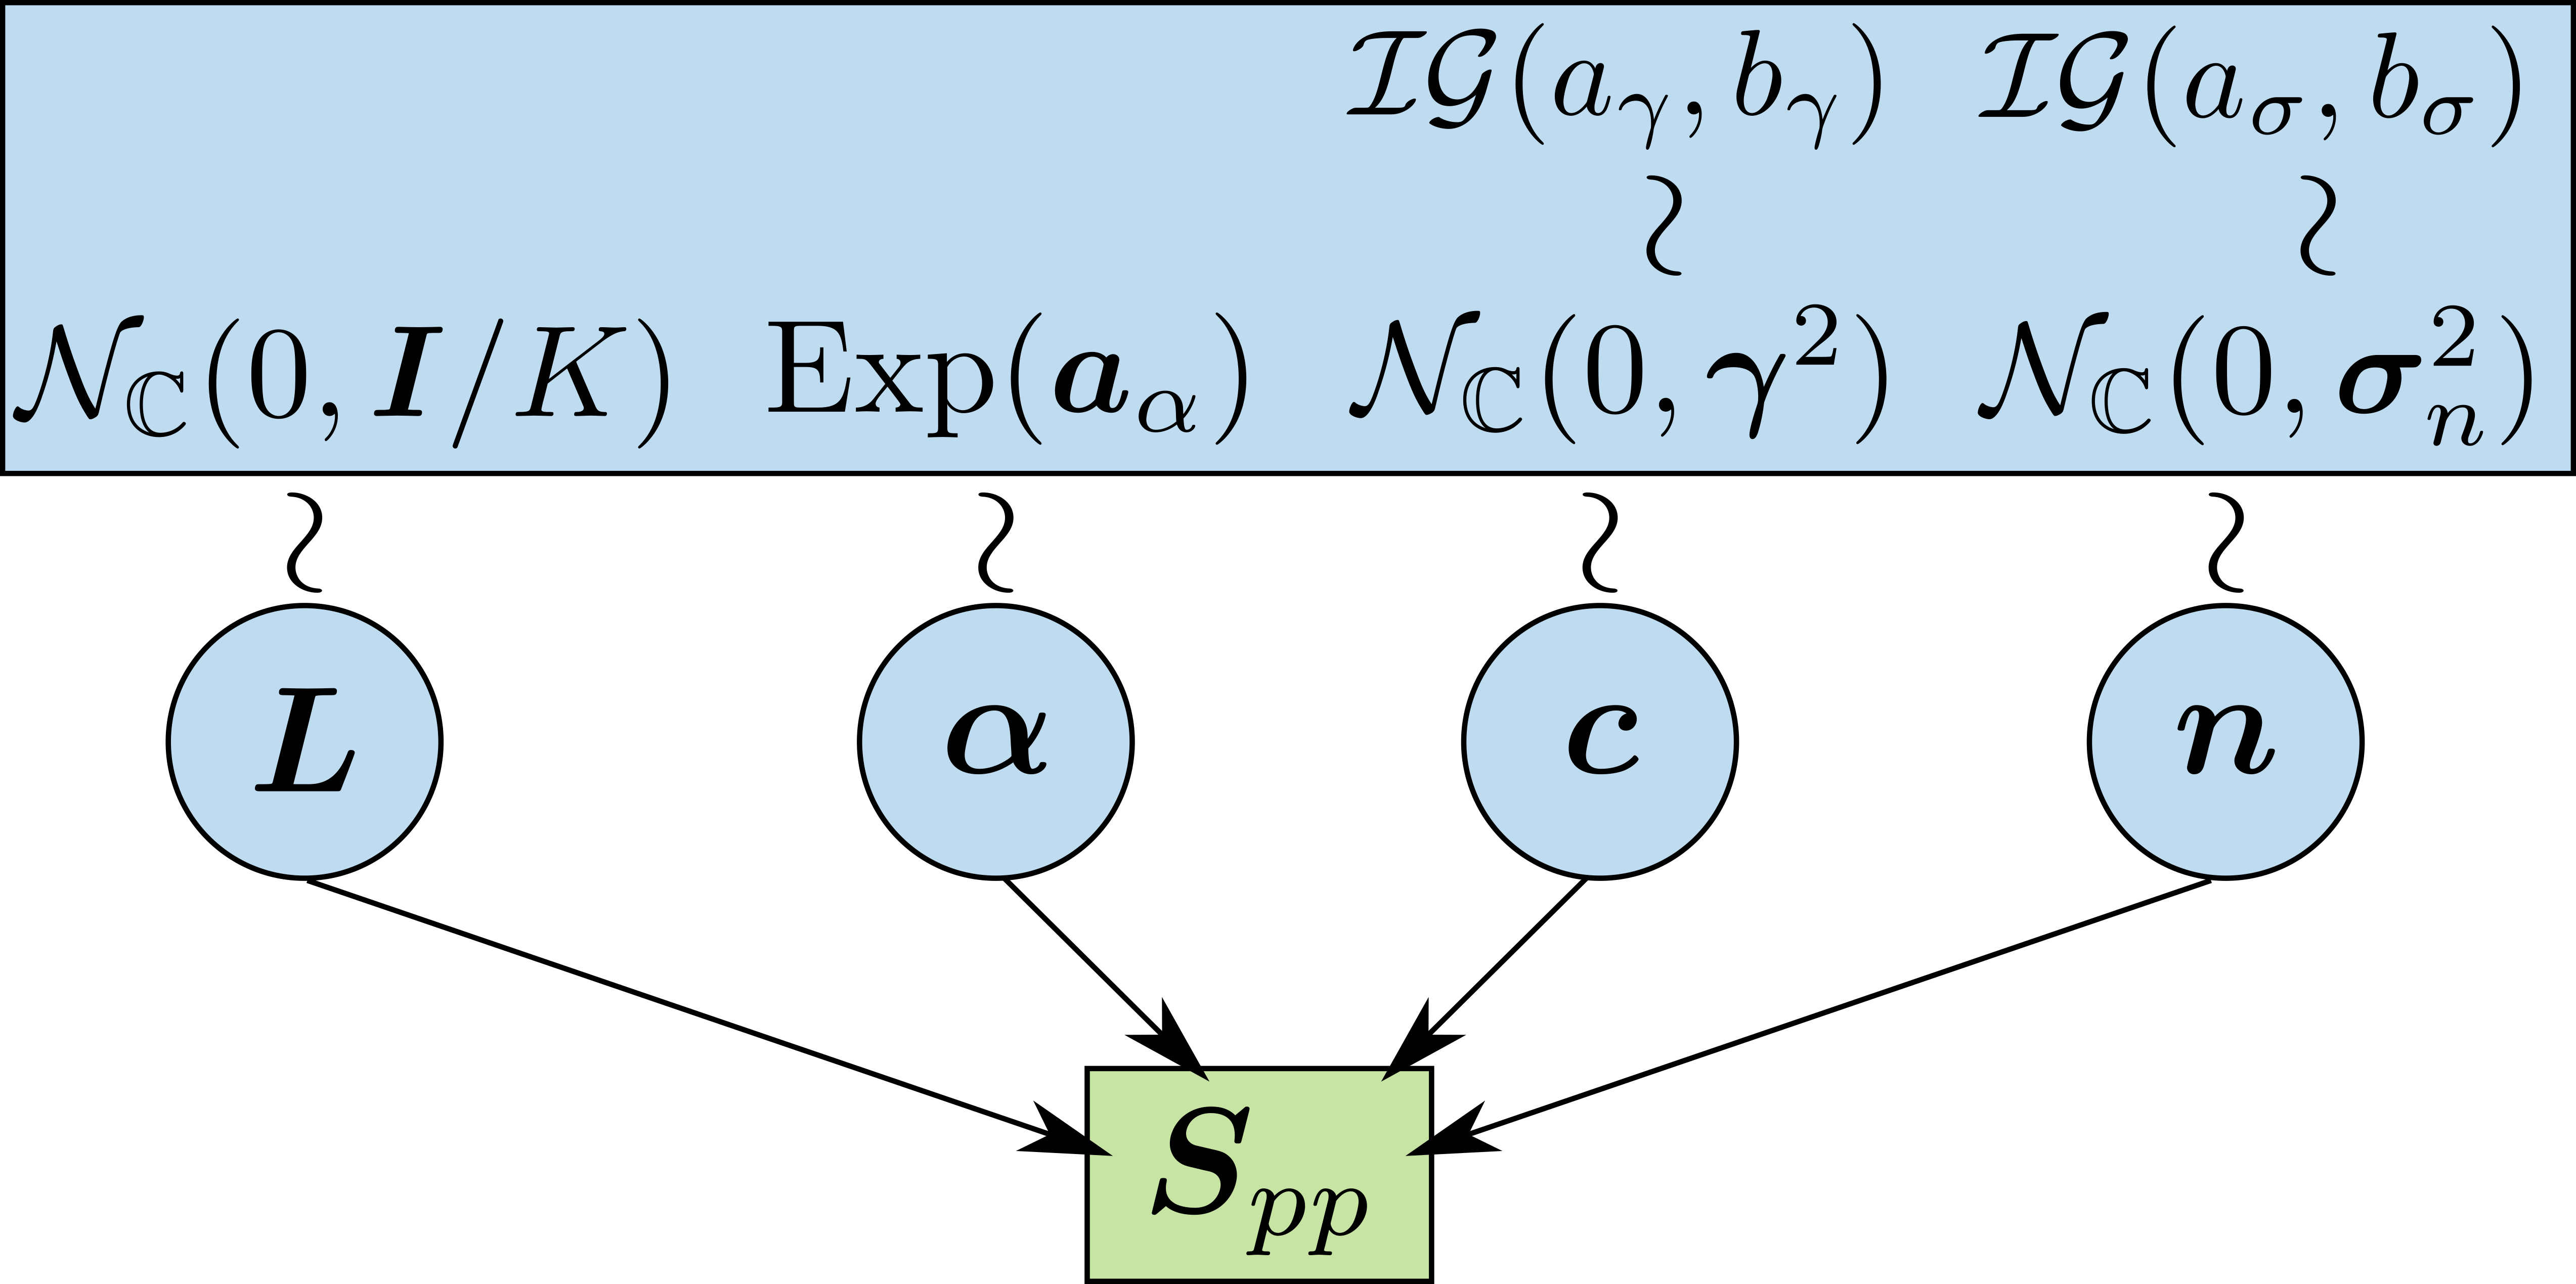
\includegraphics[width=0.5\textwidth]{img/modele.png}


\end{frame}

\begin{frame}[t]{\insertsectionhead}
\centering
{\bfseries Optimization process : maximize the posterior distribution}\\
{\itshape Find the parameter set that best fit the data}\\
\vfill
\begin{overlayarea}{\textwidth}{0.9\textheight}
\centering
\vfill
\includegraphics<4>[trim=-1.66cm 0 0 0, clip,height=0.6\textwidth,angle=-90]{img/model2.pdf}
\includegraphics<5>[trim=-1.66cm 0 0 0, clip,height=0.6\textwidth,angle=-90]{img/model0.pdf}
\includegraphics<6>[trim=-1.66cm 0 0 0, clip,height=0.6\textwidth,angle=-90]{img/model3.pdf}
\includegraphics<7>[trim=-1.66cm 0 0 0, clip,height=0.6\textwidth,angle=-90]{img/model4.pdf}
\includegraphics<8>[trim=-1.66cm 0 0 0, clip,height=0.6\textwidth,angle=-90]{img/model5.pdf}
\includegraphics<9>[trim=-1.66cm 0 0 0, clip,height=0.6\textwidth,angle=-90]{img/model6.pdf}
\includegraphics<10>[trim=-1.66cm 0 0 0, clip,height=0.6\textwidth,angle=-90]{img/model7.pdf}
\includegraphics<11>[height=0.602\textwidth,angle=-90]{img/model8.pdf}
\end{overlayarea}

\end{frame}

\begin{frame}[t]{\insertsectionhead}
\vfill
\onslide<1->{
\hspace{-0.5cm}\begin{minipage}{0.55\textwidth}
~\centerline{\resizebox{0.5cm}{!}{\circled{\textbf{+}}}} \\
\begin{itemize}
        \item[$\bullet$] MCMC:
        \begin{itemize}
   	     \item prior knowledge is part of the model
   	     \item gives credible interval
	\end{itemize}
	\item[$\bullet$] PFA:
	\begin{itemize}
   	     \item preserves CSM positivity
   	     \item reduces data dimension
   	     \item  no input parameters
   	     \item  adaptable model   	     
	\end{itemize}
\end{itemize}
\vfill
\end{minipage}
}
\hfill
\onslide<2->{
\begin{minipage}{0.45\textwidth}
~\centerline{\resizebox{0.5cm}{!}{\circled{\raisebox{-1ex}{\textbf{$\:$-$\:$}}}}}\\[1ex]
\begin{itemize}
        \item[-] Sensitive to prior choices \\ esp. for ill-posed problem
        \item[-]  Computationally expensive
\end{itemize}
\vfill
\end{minipage}
}
\vfill
\end{frame}



%\appendix
%%%% APPENDIX
%\setcounter{section}{0}
%\setbeamertemplate{headline}{%
%	\leavevmode%
%	\hbox{%
%		\begin{beamercolorbox}[wd=\paperwidth,ht=3ex,dp=1.125ex]{myheadline}%
%	   		\insertsectionnavigationhorizontal{\paperwidth}{}{}%
%	   	 \end{beamercolorbox}%
%	}
%}
%\newcounter{finalframe}
%\setcounter{finalframe}{\value{framenumber}}
%
%\section*{References}
%
%\begin{frame}{References}
%	%\begin{adjustwidth}{-2em}{-2.5em}
%		\setlength{\bibsep}{2em}
%		\bibliographystyle{abbrvnat}
%		\bibliography{biblio}
%	%\end{adjustwidth}
%\end{frame}
%


%\setcounter{framenumber}{\value{finalframe}}




%Texte du diapo \cite{Solomaa1973} et \cite{Dijkstra1982}
%\vfill
% 
%{\tiny 
%\usebibitemtemplate{\color{black}\insertbiblabel} 
%\usebibliographyblocktemplate{\color{black}}{\color{black}}{\color{black}}{\color{black}} 
% 
%\begin{thebibliography}{} 
%\bibitem{Solomaa1973} 
%A.~Salomaa. 
%\newblock {\em Formal Languages}. 
%\newblock Academic Press, 1973. 
%\bibitem{Dijkstra1982} 
%E.~Dijkstra. 
%\newblock Smoothsort, an alternative for sorting in situ. 
%\newblock {\em Science of Computer Programming}, 1(3):223--233, 1982. 
%\end{thebibliography} }


\end{document}